\documentclass[lang=cn, chinesefont=founder, math=cm, color=cyan, citestyle=gb7714-2015, bibstyle=gb7714-2015]{elegantbook}

\setmonofont{texgyrecursor}[
    UprightFont = *-regular ,
    BoldFont = *-bold ,
    ItalicFont = *-italic ,
    BoldItalicFont = *-bolditalic ,
    Extension = .otf ,
    Scale = 1.0]
\usepackage{unicode-math}
\setmathfont{STIXTwoMath-Regular.otf}

\usepackage[color=black]{siunitx}
\usepackage{tikz}
\usepackage{dashrule}
\PassOptionsToPackage{dvipsnames,svgnames,x11names}{xcolor}

\definecolor{shadow}{RGB}{210,241,241}

\newcommand{\spare}{\vspace{-1em}\begin{center}\color{structurecolor}\hdashrule[0.5ex]{\textwidth}{1pt}{1pt}\end{center}\vspace{-1em}}
\usetikzlibrary{shapes,backgrounds}
\ExecuteBibliographyOptions{sorting=gb7714-2015}
\setlength{\parskip}{1ex}
\newtcolorbox{collections}{
      boxrule=0.5pt,
      enhanced,
      breakable,
      top=8pt,
      before skip=8pt,
      colframe=structurecolor,
      colback=structurecolor!5,
      colbacktitle=structurecolor
}
\renewcommand{\bar}[1]{\overline{#1}}


\title{新世代计算机科学计划·基础篇}
\author{JouderMin}
\institute{「新世代计算机科学计划」制作委员会}
\date{\zhtoday}
\cover{img/cover.png}
\logo{img/方形logo.png}

\begin{document}
\maketitle
\frontmatter

\tableofcontents

\mainmatter

\chapter{离散数学}
\section{集合}
\begin{introduction}
    \item 集合与元素
    \item 集合的表示
    \item 子集
    \item 幂集
    \item 有序 $n$ 元组与序偶
    \item 笛卡尔积
\end{introduction}

\subsection{集合与元素}
离散数学的多数内容主要研究用以表示离散对象的离散结构,而集合则是最基础的离散结构,在本节内容中我们将了解什么是集合,以及一些与集合有关的基础概念。

以下是集合与元素的一个定义。
\begin{definition}[集合与元素]\label{def:集合与元素}
    集合是不同对象的无序聚集,这些对象也被称为集合的元素或成员。集合包含他的元素。$a \in A$ 表示 $a$ 是集合 $A$ 中的一个元素,$a \notin A$ 表示 $a$ 不是集合 $A$ 中的一个元素。
\end{definition}

我们常用大写字母表示集合,用小写字母表示元素。
\begin{definition}[相等的集合]\label{def:相等的集合}
    设有集合 $A$ 与 集合 $B$,当且仅当他们拥有相同元素时集合 $A$ 与集合 $B$ 相等,记作$A = B$。
\end{definition}

\begin{collections}
    \begin{example}
        判断下列集合是否相等。
        \begin{enumerate}
            \item $A = \{ 1, 4, 5 \}$,$B = \{ 1, 5 ,4 \}$
            \item $C = \{ \{ 1, 4 \}, 5 \}$,$D = \{ \{ 1, 5 \}, 4 \}$
            \item $E = \{ \{ 1, 4, 5 \} \}$,$F = \{ \{ 1, 5, 4 \} \}$
        \end{enumerate}
    \end{example}
    \begin{solution}
        集合 $A$ 与集合 $B$ 拥有相同的元素,所以 $A = B$;集合 $C$ 与集合 $D$ 没有相同的元素,所以 $C \neq D$;集合 $E$ 与集合 $F$ 拥有相同的元素,所以 $E = F$。
    \end{solution}
\end{collections}

集合中元素的数量被称为集合的基数,以下为基数的数学定义
\begin{definition}[集合的基数]\label{def:集合的基数}
    令 $S$ 为集合,如果集合 $S$ 中恰有 $n$ 个不同的元素($n$ 为非负整数),则称 $S$ 为有限集,$n$ 为集合 $S$ 的基数,记为 $|S|$。
\end{definition}

只有一个元素的集合叫做单元素集,单元素集的基数为 $1$;不含任何元素的集合被称为空集,记为 $\varnothing$,空集的基数为 $0$。
\begin{collections}
    \begin{example}
        判断以下集合是否空集或单元素集:
        \begin{enumerate}
            \item $A = \varnothing$
            \item $B = \{ 1 \}$
            \item $C = \{ 1, 2 \}$
            \item $D = \{ \varnothing \}$
            \item $E = \{\{ 1, 2 \}\}$
        \end{enumerate}
    \end{example}
    \begin{solution}
        集合 $A$ 是空集,因为 $|A| = 0$;集合 $B$ 是单元素集,因为 $|B| = 1$;集合 $C$ 既不是空集也不是单元素集,因为 $|C| = 2$;集合 $D$ 是单元素集,因为 $|D| = 1$;集合 $E$ 是单元素集,因为 $|E| = 1$。
    \end{solution}
\end{collections}


\subsection{集合的表示}
在离散数学中有一些常用的集合,一般用黑体大写字母表示。
\begin{itemize}
    \item $\symbf{N}$ 为所有自然数的集合;
    \item $\symbf{Z}$ 为所有整数的集合;
    \item $\symbf{Z}^+$ 为所有正整数的集合;
    \item $\symbf{Q}$ 为所有有理数的集合;
    \item $\symbf{R}$ 为所有实数的集合;
    \item $\symbf{C}$ 为所有复数的集合。
\end{itemize}

描述集合有多种方式,人们常用以下三种方式来表示集合:
\begin{itemize}
    \item 花名册方法(俗称枚举法);
    \item 集合构造器符号(俗称描述法);
    \item 文氏图。
\end{itemize}

花名册方法,俗称枚举法,这种方法需要在可能的情况下一一列出集合中的元素。在集合中关系显然的情况下,可以用 $\cdots$ 省略部分元素。
\begin{collections}
    \begin{example}
        使用花名册方法表示小于 $10$ 的正素数集合 $O$ 。
    \end{example}
    \begin{solution}
        $O = \{ 2, 3, 5, 7 \}$
    \end{solution}

    \spare

    \begin{example}
        使用花名册方法表示小于等于 $100$ 的所有自然数集合 $Q$。
    \end{example}
    \begin{solution}
        $Q = \{ 0, 1, 2, \cdots, 100 \}$
    \end{solution}
\end{collections}

我们也可以使用集合构造器符号来表示集合,这种方法俗称描述法,需要描述集合中元素必须具有的性质。一般采用记号 $\{x \mid x\text{\,具有性质\,}P\}$。
\begin{collections}
    \begin{example}
        使用集合构造器符号表示大于等于 $10$,小于 $100$ 的正整数集合 $P$ 。
    \end{example}
    \begin{solution}
        $P=\{x \in Z^+ \mid 10 \leq x < 100\}$
    \end{solution}
\end{collections}

集合也可以用文氏图来表示。在文氏图中,全集 $U$ 包含所考虑的所有元素,用矩形框表示,矩形框中的圆形或其他几何形状用于表示集合,点表示集合中的元素。文氏图常用来表示集合之间的关系。
\begin{collections}
    \begin{example}
        设集合 $A$ 包含在全集 $U$ 中,用文氏图表示集合 $A$ 与全集 $U$。
    \end{example}
    \begin{solution}
        \begin{center}
            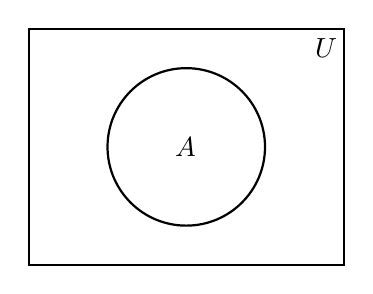
\begin{tikzpicture}
                \draw[thick] (0,0) rectangle (4,3);
                \draw[thick] (2,1.5) circle (1);

                \node[below left] at (4,3) {$U$};
                \node at (2,1.5) {$A$};
            \end{tikzpicture}
        \end{center}
    \end{solution}
\end{collections}

\subsection{子集}
子集是集合之间的一种关系。
\begin{definition}[子集与超集]\label{def:子集与超集}
    当且仅当集合 $A$ 中的所有元素都是集合 $B$ 的元素时,集合 $A$ 称为集合 $B$ 的子集,记作 $A \subseteq B$,集合 $B$ 称为集合 $A$ 的超集,记作 $B \supseteq A$。
\end{definition}

在文氏图中可以直观表示子集关系。设集合 $B$ 是集合 $A$ 的子集,集合 $U$ 是全集,则可以作出图 \ref{fig:子集文氏图}。
\begin{figure}[htbp!]
    \centering
    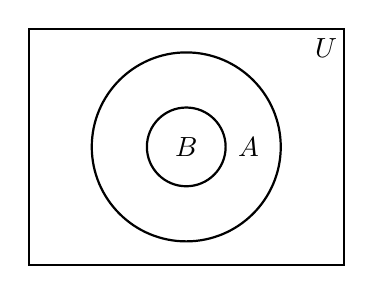
\begin{tikzpicture}
        \draw[thick] (0,0) rectangle (4,3);
        \draw[thick] (2,1.5) circle (1.2);
        \draw[thick] (2,1.5) circle (0.5);

        \node[below left] at (4,3) {$U$};
        \node at (2,1.5) {$B$};
        \node at (2.8,1.5) {$A$};
    \end{tikzpicture}
    \caption{表示 $B \subseteq A$ 的文氏图}
    \label{fig:子集文氏图}
\end{figure}

子集关系有以下定理:
\begin{theorem}\label{thm:集合与空集之间的关系}
    对任意集合 $S$,总有 $\varnothing \subseteq S$。
\end{theorem}

\begin{theorem}\label{thm:集合与其自身的关系}
    对任意集合 $S$,总有 $S \subseteq S$。
\end{theorem}

定理 \ref{thm:集合与其自身的关系} 可以用于证明两个集合是否相等。
\begin{theorem}\label{thm:证明集合相等}
    对于集合 $A$,如果存在集合 $B$ 使 $A \subseteq B$ 与 $B \subseteq A$ 成立,则 $A = B$。
\end{theorem}

\subsection{幂集}
\begin{definition}[幂集的定义]\label{def:幂集的定义}
    给定集合 $S$,$S$ 的幂集是集合 $S$ 所有子集的集合,$S$ 的幂集记为 $\symcal{P}(S)$ 或 $2^S$。
\end{definition}

\begin{collections}
    \begin{example}
        求以下集合的幂集。
        \begin{enumerate}
            \item $A = \{1, 2, 3\}$
            \item $B = \{ \varnothing \}$
            \item $C = \{\{ \varnothing \}\}$
        \end{enumerate}
    \end{example}
    \begin{solution}
        \begin{enumerate}
            \item $\symcal{P}(A) = \{\varnothing, 1, 2, 3, \{1, 2\}, \{1, 3\}, \{2, 3\}, \{1, 2, 3\}\}$
            \item $\symcal{P}(B) = \{\varnothing\}$
            \item $\symcal{P}(C) = \{\varnothing, \{\varnothing\}\}$
        \end{enumerate}
    \end{solution}
\end{collections}

\begin{theorem}
    令 $S$ 为集合,设 $|S| = n$,则$|\symcal{P}(S)| = 2^n$。
\end{theorem}

\subsection{有序 $n$ 元组与序偶}
集合中的元素是无序排列的,所以我们需要一种结构来表示有序的聚集,这便是有序 $n$ 元组。
\begin{definition}[有序 $n$ 元组与序偶]\label{def:有序n元组与序偶}
    有序 $n$ 元组 $(a_1, a_2, \cdots, a_n)$ 是以 $a_1$ 为第 $1$ 个元素,$a_2$ 为第 $2$ 个元素,$\cdots$,$a_n$ 为第 $n$ 个元素的有序聚集。特别的,有序二元组被称为序偶。
\end{definition}

两个有序 $n$ 元组相等当且仅当每一对对应的元素相等。
\begin{collections}
    \begin{example}
        判断 $A=(1, 2)$ 与 $B=(2, 1)$ 是否相等。
    \end{example}
    \begin{solution}
        $A \neq B$
    \end{solution}
\end{collections}

\subsection{笛卡尔积}
\begin{definition}[笛卡尔积]\label{def:笛卡尔积}
    令 $A$ 和 $B$ 为集合,$A$ 与 $B$ 的笛卡尔积(记作 $A \times B$)是所有序偶 $(a,b)$ 的集合,其中 $a \in A$ 且 $b \in B$。
    \begin{equation*}
        A \times B = \{(a,b) \mid a \in A \land b \in B \}
    \end{equation*}
\end{definition}

\begin{collections}
    \begin{example}
        已知$A = \{1, 2\}$,$B = \{a, b, c\}$,求 $A \times B$ 和 $B \times A$。
    \end{example}
    \begin{solution}
        $$A \times B = \{(1, a), (1, b), (1, c), (2, a), (2, b), (2, c)\}$$
        $$B \times A = \{(a, 1), (a, 2), (b, 1), (b, 2), (c, 1), (c, 2)\}$$
    \end{solution}
\end{collections}

%TODO 准备例题
\section{集合的运算}
\begin{introduction}
    \item 交集
    \item 并集
    \item 差集
    \item 补集
    \item 对称差
\end{introduction}

\subsection{交集}
\begin{definition}[集合的交集]\label{def:交集}
    令 $A$ 与 $B$ 为集合。集合 $A$ 与 $B$ 的交集是一个集合,它包含集合 $A$ 与 $B$ 中共有的元素,记作 $A \cap B$。
    \begin{equation*}
        A \cap B = \{x \mid x \in A \land x \in B \}
    \end{equation*}
\end{definition}

集合 $A$ 与 $B$ 的交集可以用图 \ref{fig:交集文氏图} 中的阴影部分表示。
\begin{figure}[htbp!]
    \centering
    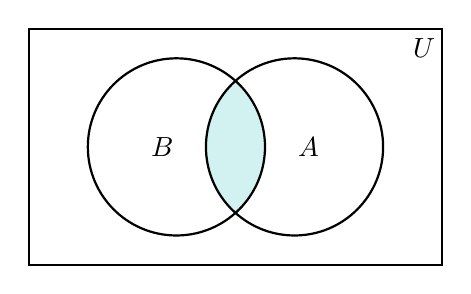
\begin{tikzpicture}[scale=0.75]
        \begin{scope}
            \clip (2,2) circle (1.5);
            \fill[shadow] (4,2) circle (1.5);
        \end{scope}

        \draw[thick] (-0.5,0) rectangle (6.5,4);
        \draw[thick] (2,2) circle (1.5);
        \draw[thick] (4,2) circle (1.5);

        \node[below left] at (6.5,4) {$U$};
        \node at (1.75,2) {$B$};
        \node at (4.25,2) {$A$};
    \end{tikzpicture}
    \caption{$A \cap B$ 的文氏图}
    \label{fig:交集文氏图}
\end{figure}

由此我们还可以定义一组集合的交集。
\begin{definition}[多个集合的交集]\label{def:多个交集}
    一组集合的交集是包含这组集合中所有成员集合共有的元素的集合。
\end{definition}

我们用符号
\begin{equation*}
    \bigcap_{i=1}^n A_i=A_1 \cap A_2 \cap \cdots \cap A_i
\end{equation*}
表示 $A_1$,$A_2$,$\cdots$,$A_n$ 的交集。

\subsection{并集}
\begin{definition}[集合的并集]\label{def:并集}
    令 $A$ 与 $B$ 为集合。集合 $A$ 与 $B$ 的并集是一个集合,它包含 $A$ 和 $B$ 中的所有元素,记作 $A \cup B$。
    \begin{equation*}
        A \cup B = \{x \mid x \in A \lor x \in B\}
    \end{equation*}
\end{definition}

集合 $A$ 与 $B$ 的并集可以用图 \ref{fig:并集文氏图} 中的阴影部分表示。
\begin{figure}[htbp!]
    \centering
    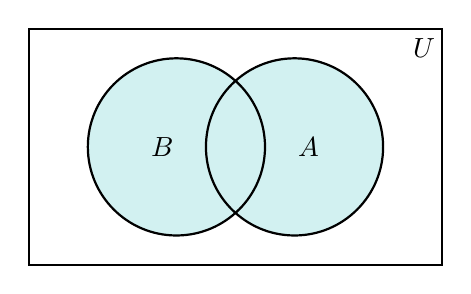
\begin{tikzpicture}[scale=0.75]
        \begin{scope}
            \clip (2,2) circle (1.5);
            \fill[shadow] (4,2) circle (1.5);
        \end{scope}
        \begin{scope}
            \clip (2,2) circle (1.5) (-0.5,0) rectangle (6.5,4);
            \fill[shadow] (4,2) circle (1.5);
        \end{scope}
        \begin{scope}
            \clip (4,2) circle (1.5) (-0.5,0) rectangle (6.5,4);
            \fill[shadow] (2,2) circle (1.5);
        \end{scope}

        \draw[thick] (-0.5,0) rectangle (6.5,4);
        \draw[thick] (2,2) circle (1.5);
        \draw[thick] (4,2) circle (1.5);

        \node[below left] at (6.5,4) {$U$};
        \node at (1.75,2) {$B$};
        \node at (4.25,2) {$A$};
    \end{tikzpicture}
    \caption{$A \cup B$ 的文氏图}
    \label{fig:并集文氏图}
\end{figure}

同交集一样,由此我们还可以定义一组集合的并集。
\begin{definition}[多个集合的并集]\label{def:多个并集}
    一组集合的交集是包含这组集合中所有成员集合的元素的集合。
\end{definition}

我们用符号
\begin{equation*}
    \bigcup_{i=1}^n A_i=A_1 \cup A_2 \cup \cdots \cup A_i
\end{equation*}
表示 $A_1$,$A_2$,$\cdots$,$A_n$ 的并集。

\subsection{差集}
\begin{definition}[集合的差集]\label{def:差集}
    令 $A$ 与 $B$ 为集合,集合 $A$ 和 $B$ 的差集是一个集合,它包含属于 $A$ 但不属于 $B$ 的元素,记作 $A-B$。
    \begin{equation*}
        A - B = \{ x \mid x \in A \land x \notin B \}
    \end{equation*}
\end{definition}

集合 $A$ 与 $B$ 的差集可以用图 \ref{fig:差集文氏图} 中的阴影部分表示。
\begin{figure}[htbp!]
    \centering
    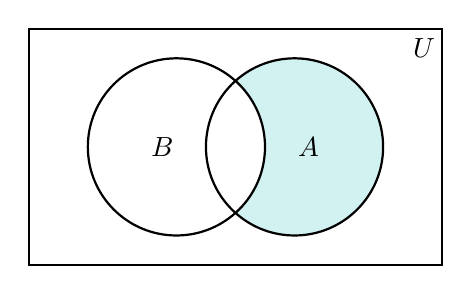
\begin{tikzpicture}[scale=0.75]
        \begin{scope}
            \clip (2,2) circle (1.5) (-0.5,0) rectangle (6.5,4);
            \fill[shadow] (4,2) circle (1.5);
        \end{scope}

        \draw[thick] (-0.5,0) rectangle (6.5,4);
        \draw[thick] (2,2) circle (1.5);
        \draw[thick] (4,2) circle (1.5);

        \node[below left] at (6.5,4) {$U$};
        \node at (1.75,2) {$B$};
        \node at (4.25,2) {$A$};
    \end{tikzpicture}
    \caption{$A - B$ 的文氏图}
    \label{fig:差集文氏图}
\end{figure}

\subsection{补集}
\begin{definition}[集合的补集]
    令 $U$ 为全集,集合 $A$ 的补集就是 $U-A$,记作 $\bar{A}$
\end{definition}

集合 $A$ 的补集可以用图 \ref{fig:补集文氏图} 中的阴影部分表示。
\begin{figure}[htbp!]
    \centering
    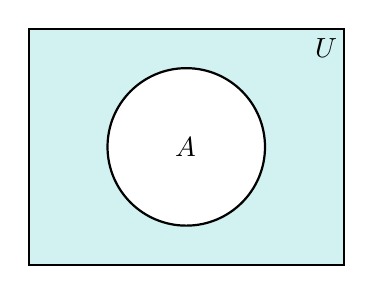
\begin{tikzpicture}
        \begin{scope}
            \clip (0,0) rectangle (4,3) (2,1.5) circle (1);
            \fill[shadow] (0,0) rectangle (4,3);
        \end{scope}
        \draw[thick] (0,0) rectangle (4,3);
        \draw[thick] (2,1.5) circle (1);

        \node[below left] at (4,3) {$U$};
        \node at (2,1.5) {$A$};
    \end{tikzpicture}
    \caption{$\bar{A}$ 的文氏图}
    \label{fig:补集文氏图}
\end{figure}

\subsection{对称差}
\begin{definition}[集合的对称差]\label{def:对称差}
    令 $A$ 与 $B$ 为集合,集合 $A$ 与 $B$ 的对称差是一个集合,由属于 $A$ 但不属于 $B$ 和属于 $B$ 但不属于 $A$ 的元素组成,记作 $A \oplus B$。
\end{definition}

集合 $A$ 与 $B$ 的对称差可以用图 \ref{fig:对称差文氏图} 中的阴影部分表示。
\begin{figure}[htbp!]
    \centering
    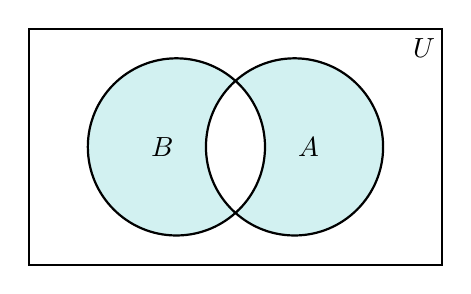
\begin{tikzpicture}[scale=0.75]
        \begin{scope}
            \clip (2,2) circle (1.5) (-0.5,0) rectangle (6.5,4);
            \fill[shadow] (4,2) circle (1.5);
        \end{scope}
        \begin{scope}
            \clip (4,2) circle (1.5) (-0.5,0) rectangle (6.5,4);
            \fill[shadow] (2,2) circle (1.5);
        \end{scope}

        \draw[thick] (-0.5,0) rectangle (6.5,4);
        \draw[thick] (2,2) circle (1.5);
        \draw[thick] (4,2) circle (1.5);

        \node[below left] at (6.5,4) {$U$};
        \node at (1.75,2) {$B$};
        \node at (4.25,2) {$A$};
    \end{tikzpicture}
    \caption{$A \oplus B$ 的文氏图}
    \label{fig:对称差文氏图}
\end{figure}
\end{document}